\documentclass[../document.tex]{subfiles}
\begin{document}
\chapter{Methodology}
\begin{figure}[H]
    \centering
        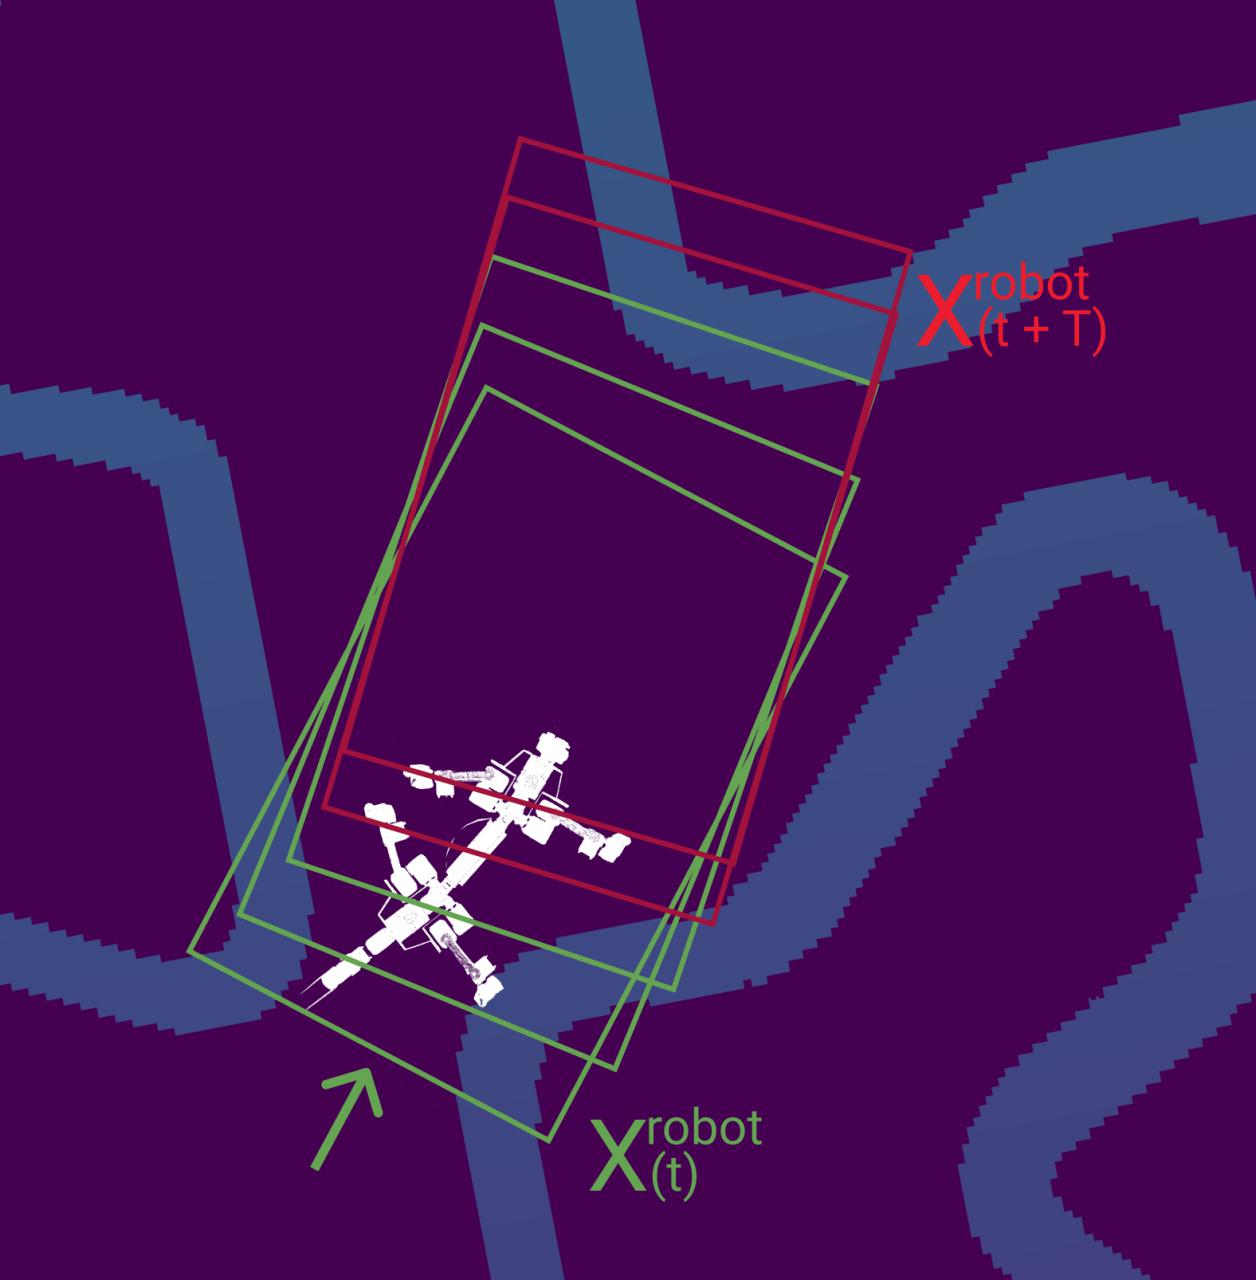
\includegraphics[width=\textwidth]{../img/krock-bars-correct.jpg}
    \caption{Example of a robot trajectory extracted during training from \emph{bars1}. Robot's initial position is showed by its white siluette. Patches borders are label with greed if traversable and red if not.}
    \end{figure}
\end{document}